% Created 2024-09-16 Mon 11:23
% Intended LaTeX compiler: pdflatex
\documentclass[10pt]{article}
% =================================BASE====================================%
\usepackage[left=2cm,right=2cm,top=2cm,bottom=2cm]{geometry} % Marges
\usepackage[T1]{fontenc} % Nécessaire avec FrenchBabel
\usepackage[utf8]{inputenc} % Important pour symboles Francophones, é,à,etc
\usepackage{csquotes} % Recommandé par PDFLatex lors de la compilation. 

% Calligraphie
%\usepackage{pxfonts} % Met le texte ET les maths en Palatino + donne accès à des symboles math
%\usepackage{palatino} % Cette commande met seulement le texte en police palatino
\usepackage{lmodern} % Pour les maths? Lmodern pour les maths
\usepackage{cfr-lm}
% Use lmodern for sans-serif
\usepackage{mathrsfs} % Permet la command \mathscr (Lettres attachées genre) \mathscr(ABC)
\usepackage{eucal}   % Vient changer le \mathcal{ABC} parce que celui de base est laid.

% Bibliographie
\usepackage[backend=biber,style=alphabetic,sorting=ynt,maxbibnames=99]{biblatex}
%\usepackage[backend=biber,sorting=ynt,style=authoryear]{biblatex} % Ça semble tout changer.
\addbibresource{master-bibliography.bib}


\usepackage{amsmath, amssymb, amsthm} % Symb. math. (Mathmode+Textmode) + Beaux théorèmes.
\usepackage{mathtools,cancel,xfrac} % Utilisation de boîtes \boxed{} + \cancelto{}{}, xfrac
\usepackage{graphicx, wrapfig} % Géstion des figures.
\usepackage{hyperref} % Permettre l'utilisation d'hyperliens.
\usepackage{color} % Permettre l'utilisation des couleurs.
\usepackage{colortbl} % Color tables
\usepackage[dvipsnames]{xcolor} % Couleurs avancées.

% Physique
\usepackage{physics} % Meilleur package pour physicien. 

% Style
\usepackage{lipsum} % For fun
\usepackage{tikz} % Realisation de figures TIKZ.
\usetikzlibrary{arrows.meta,bending, shapes.geometric, automata, positioning} % Arrow heads et les formes de noeuds
\usepackage{empheq} % Boite autour de MULTIPLE équations
\usepackage{bbding}

% Français
\usepackage[french]{babel} % Environnements en Français.

\usepackage{titling} % Donne accès à \theauthor, \thetitle, \thedate
% ==============================BASE-(END)=================================%





% ================================SETTINGS=================================%
% Pas d'indentation en début de paragraphe :
\setlength\parindent{0pt}
\setlength{\parskip}{0.15cm}

% Tableaux/tabular
% Espace vertical dans les tabular/tableaux
\renewcommand{\arraystretch}{1.2}
% Couleur des tableaux/tabular
% \rowcolors{3}{violet!5}{}

% Couleurs de hyperliens :
\definecolor{mypink}{RGB}{147, 0, 255}
\hypersetup{colorlinks, 
             filecolor=mypink,
             urlcolor=mypink, 
             citecolor=mypink, 
             linkcolor=mypink, 
             anchorcolor=mypink}


% Numéros d'équations suivent les sections :
\numberwithin{equation}{section} 

% Les « captions » sont en italique et largeur limitée
\usepackage[textfont = it]{caption} 
\captionsetup[wrapfigure]{margin=0.5cm}

% Retirer l'écriture en gras dans la table des matières
\usepackage{tocloft}
\renewcommand{\cftsecfont}{\normalfont}
\renewcommand{\cftsecpagefont}{\normalfont}


% On a des lignes à droite des sections et sous-sections
\usepackage[explicit]{titlesec}
    % Raised Rule Command:
    % Arg 1 (Optional) - How high to raise the rule
    % Arg 2 - Thickness of the rule
    \newcommand{\raisedrulefill}[2][0ex]{\leaders\hbox{\rule[#1]{1pt}{#2}}\hfill}
    \titleformat{\section}{\Large\bfseries}{\thesection. }{0em}{#1\;\raisedrulefill[0.4ex]{0.25pt}}
    \titleformat{\subsection}{\large\bfseries}{\thesubsection. }{0em}{#1\;\raisedrulefill[0.4ex]{0.10pt}}


% Change bullet style
%\usepackage{pifont}
\usepackage{enumitem}
%\setlist[itemize,1]{label=\ding{224}}
%\setlist[itemize,1]{label=\ding{239}}
%\setlist[itemize,1]{label=$\cdot$}
\renewcommand{\boxtimes}{\blacksquare}
% ================================SETTINGS=================================%



% ==============================NEWCOMMANDS================================%
% CQFD symbol
\renewcommand{\qedsymbol}{$\hfill\blacksquare$}
\newcommand{\cqfd}{\hfill$\blacktriangleleft$}

% Vecteurs de base :
\newcommand{\nvf}{\vb{\hat{n}}}
\newcommand{\evf}{\vb{\hat{e}}}
\newcommand{\ivf}{\vb{\hat{i}}}
\newcommand{\jvf}{\vb{\hat{j}}}
\newcommand{\kvf}{\vb{\hat{k}}}
\newcommand{\uu}{\vb{u}}
\newcommand{\vv}{\vb{v}}
\newcommand{\ust}{\vb{u}_{\ast}}
\newcommand{\xx}{\vb{x}}
\newcommand{\rad}{\text{Rad}}

% Physics empty spaces 
\newcommand{\short}{\vphantom{pA}}
\newcommand{\tall}{\vphantom{pA^{x^x}_p}}
\newcommand{\grande}{\vphantom{\frac{1}{xx}}}
\newcommand{\venti}{\vphantom{\sum_x^x}}
\newcommand{\pt}{\hspace{1pt}} % One horizontal pt space

% Moyenne numérique entre deux points de grilles. 
\newcommand{\xmean}[1]{\overline{#1}^x}
\newcommand{\ymean}[1]{\overline{#1}^y}
\newcommand{\zmean}[1]{\overline{#1}^z}
\newcommand{\xymean}[1]{\overline{#1}^{xy}}

% Tilde over psi
\newcommand{\tpsi}{\tilde{\psi}}
\newcommand{\tphi}{\tilde{\phi}}

% Nota Bene env : (\ding{89})
%\newcommand{\nb}{$\boxed{\text{\footnotesize\EightStarConvex}\pt \mathfrak{N. B.}}$\hspace{4pt}}
\newcommand{\nb}{\underline{{\footnotesize\EightStarConvex}\pt $\mathfrak{N.B.}$\vphantom{p}}\hspace{3pt}}

\newcommand{\exemple}{
\parbox[center]{2.2cm}{\begin{tcolorbox}[sharp corners, rounded corners=northeast, rounded corners=southeast,
colback=Violet!2, colframe=black,
size=small, width=2cm, left=-0.25pt, bottom=-0.5pt,
arc is angular, arc=2.5mm, boxrule=0.35pt, leftrule=4pt, %bottomrule=1pt,
after={\enskip}] Exemple \end{tcolorbox}}}

% Define the nota bene environment
\usepackage{tcolorbox}
\newtcolorbox{notabene}{
     colback=blue!5,
     colframe=black,
     boxrule=0.5pt,
     arc=2pt,
     left=5pt,
     right=5pt,
     top=5pt,
     bottom=5pt,
}


\newcommand{\cmark}{\ding{52}}
\newcommand{\xmark}{\ding{55}}

%\newcommand{\fourier}[1]{\raisebox{-0.4em}{\resizebox{2em}{!}{$\mathscr{F}$}\,}\qty[#1]}
\newcommand{\fourier}{\operatorname{\raisebox{-0.4em}{\resizebox{2em}{!}{$\mathscr{F}$}}}}
% Mettre (a,b) à la suite d'une série d'équations horizontales.
\newcommand{\ab}{\refstepcounter{equation}\tag{\theequation a,b}}
% ==============================NEWCOMMANDS================================%



% ==============================PAGE-TITRE=================================%
% Titlepage 
\newcommand{\mytitlepage}{
\begin{titlepage}
\begin{center}
{\Huge \thesubtitle \par}
\vspace{2cm}
{\Huge \MakeUppercase{\thetitle} \par}
\vspace{2cm}
RÉALISÉ DANS LE CADRE\\ D'UN PROJET POUR \par
\vspace{2cm}
{\Huge ISMER--UQAR \par}
\vspace{2cm}
{\thedate}
\end{center}
\vfill
Rédaction \\
{\theauthor}\\
\url{charles-edouard.lizotte@uqar.ca}\\
ISMER-UQAR\\
Police d'écriture : \textbf{CMU Serif Roman}
\end{titlepage}
}
% ==============================PAGE-TITRE=================================%



% =================================ENTÊTE==================================%
\usepackage{fancyhdr}
\pagestyle{fancy}
\setlength{\headheight}{13pt}
\renewcommand{\headrulewidth}{0.0pt} % Ligne horizontale en haut

\fancyhead[R]{\underline{\textit{Section \thesubsection}}}
\fancyhead[L]{\underline{\textit{\thepage}}}
\fancyfoot[R]{\textit{\theauthor}}
\fancyfoot[L]{}
\fancyfoot[C]{} 
% =================================ENTÊTE==================================%
\author{Charles-Édouard Lizotte}
\date{30/08/2024}
\title{Rapport hebdomadaire}
\newcommand{\thesubtitle}{Contrat Été 2024}
\hypersetup{
 pdfauthor={Charles-Édouard Lizotte},
 pdftitle={Rapport hebdomadaire},
 pdfkeywords={},
 pdfsubject={},
 pdfcreator={Emacs 29.4 (Org mode 9.7.8)}, 
 pdflang={French}}
\begin{document}

\mytitlepage
\tableofcontents\newpage
\section{Recherche d'une variable d'hétérogénéité}
\label{sec:org8bc5a62}

\subsection{Retour sur les travaux de Bismuth}
\label{sec:org6db6661}

\begin{figure}[htbp]
\centering
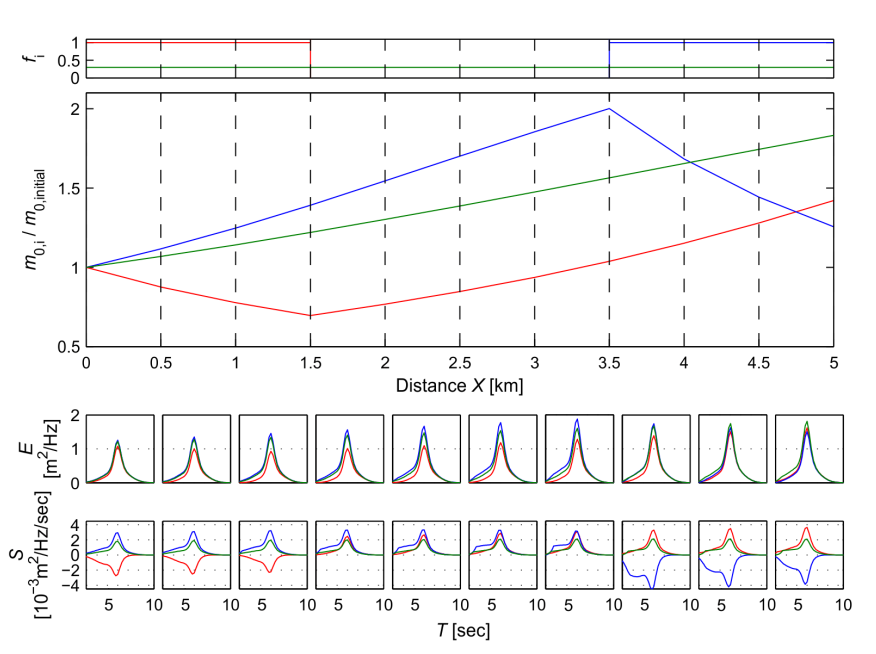
\includegraphics[width=.9\linewidth]{Figures/figures/Bismuth-fig13.png}
\caption{Figure tirée de Bismuth (figure 13) représentant les termes sources actifs et la prédominance de chacun.}
\end{figure}

\begin{figure}[htbp]
\centering
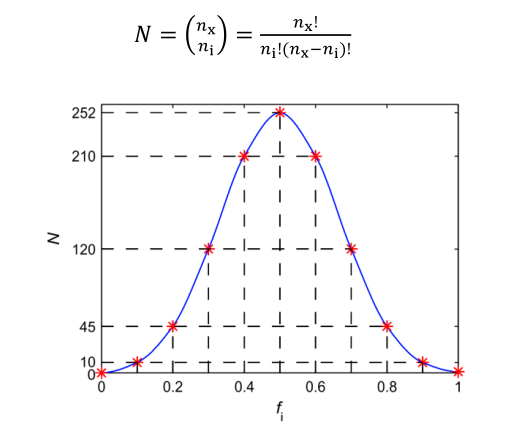
\includegraphics[width=.9\linewidth]{Figures/figures/Bismuth-fig10.png}
\caption{Distribution statistique représentant le nombre possible de distribution de glace associé à chaque "concentration" \(f_i\) dans un domaine de 10 cases (\(2^8\)).}
\end{figure}

Grossièrement, il y a un concept qui s'appelle l'entropie de Shanon.
Cette dernière est définie comme
\begin{equation}
\label{eq:org3f99cc5}
   H(\mathcal{X}) = -\sum_i^n p(x_i) \log_b[\pt p(x_i)\pt]
\end{equation}
où l'indice «\textit{b}» est 2, faisant référence au concept de \emph{bit} d'information; \(p(x_i)\) est la probabilité d'avoir une valeur désirée au point \(x_i\); \(\mathcal{X}\) est notre variable aléatoire.\bigskip

Pour une distribution complétement aléatoire, on aurait tout simplement la distribution de Bernouilli, donc ce qui est illustré plus haut.
On peut calculer son entropie de Shanon à l'aide de l'équation \ref{eq:org3f99cc5}, soit
\begin{equation}
   H(\mathcal{X}) = -\sum_i^n \qty(\frac{1}{2}) \log_2\qty[\frac{1}{2}] = \frac{n}{2}\cdot (-1) = \frac{-n}{2}.
\end{equation}
Par contre, ça devient intéressant quand on vient modifier la distribution des floes.
On pourrait aisément dire que les probabilité augmentent de manière linéaire, donc
\begin{equation}
   p(x_i) = \frac{x_i}{L_x}
\end{equation}
\subsection{Retour sur les distributions statistiques de glace}
\label{sec:orgb40faa4}

On a une distribution d'épaisseurs \(g(h)\) qui est définit de sorte à ce que \(g(h)\dd h\) est la
fraction de l'aire couvert pas la glace d'épaisseur entre \(h\) et \(\dd h\) dans une cellule de grille.\bigskip

Prenons l'exemple de la figure \ref{org1561c2f}, on y retrouve une distribution spatiale d'épaisseur sur une case à gauche; puis à droite une distribution de l'aire couvert par chaque tranche d'épaisseur.

\begin{figure}[h]
\begin{center}
\begin{tikzpicture}
   \fill[Aquamarine!5] (0,0) rectangle (3,3);
   \draw[dashed] (0,0) rectangle (3,3);
   \fill[left color=blue!30, right color = violet] (0,0) -- (3,3) -- (3,0);
   \draw (-0.25,-0.25) node [] {$0$};
   \draw[] (0,1.6) node [left] {$\Delta {y}$};
   \draw[] (1.6,0) node [below] {$\Delta {x}$};
   \draw[] (1.6,3.5) node [] {$h(x)=\qty(\frac{h_p}{\Delta x})\pt x$};
   \draw[] (1,2) node [RoyalBlue!50!black] {Eau};
   \draw[] (2,1) node [white] {Glace};
   \fill[bottom color=blue!30, top color = violet] (3.2,0) rectangle (3.4,3);
   \draw (3.4,1.5) node [right] {$h$};
\end{tikzpicture}\hspace{1cm}\begin{tikzpicture}
   \draw[black, dotted] (0,0) grid (3,3);
   \filldraw[draw=Periwinkle, fill=blue!5 ,thick] (0,0) -- (3,3) -- (3,0);
   \draw (-0.25,-0.25) node [] {$0$};
   \draw[-latex] (0,0) -- (0,3.2) node [left] {$g(h)$};
   \draw[-latex] (0,0) -- (3.2,0) node [below] {$h$};
   \fill[Periwinkle!80] (2.1,0) -- (2.1,2.1) -- (2.5,2.5) -- (2.5,0);
   \draw (2.3,0) node[below, Periwinkle] {$\var h$};
   \draw[] (1.4,3.5) node [] {$g(h) = \frac{h}{h_p^2}$};
\end{tikzpicture}
\end{center}
\caption{\label{org1561c2f}À gauche, Couvert de glace d'une cellule. À droite distribution de l'aire}
\end{figure} 

Dany m'a aussi reparlé de la distribution \(J\).
Cette distribution est en fait une genre d'équation d'état, mais statistique.
Elle représente en fait une \emph{flow size and thickness distribution} \autocite{dumont2022marginal}, soit
\begin{equation}
   J(r,h) = J(\vb{r})
\end{equation}
\section{Rencontre avec Dany mercredi [2/3]}
\label{sec:orgb1b5469}

\emph{Grosso modo}, Dany a proposé \textbf{trois axes importants} pour cette semaine :
\begin{itemize}
\item[{$\square$}] Lire sur l'inégalité de Jensen;
\item[{$\boxtimes$}] Bien poser le problème par rapport à l'hétérogénéité des amas de glaces dans un point de grille global;
\item[{$\boxtimes$}] Résoudre le problème de la trainée spectrale à l'aide des notes de Sebastien Dugas (Réalisé à moitié)
\end{itemize}
\subsection{Lire un peu sur l'inégalité de Jensen}
\label{sec:orge4ff1c5}
J'ai tout simplement pas eu le temps, malheureusement.
\subsection{Bien poser le problème pour la présentation du 9 septembre}
\label{sec:org9084f81}
Dany suggère de \textbf{bien poser le problème}, ce sera super important.
Car pour l'instant, il faut mentionner que le \emph{challenge} c'est de caractériser la distribution sous-grille.
De plus, ça serait important de mentionner qu'il y a un lien entre les vagues et la glace -- ce qui justifierait justement notre étude.
Donc, faut pas avoir peur de citer le \emph{power} \emph{point} de Dany.\bigskip


Grossièrement, la séquence optimale devrait être celle ci : 

\begin{center}    
\begin{tikzpicture}[node distance = 2cm]
   \tikzstyle{concept} = [rectangle, rounded corners, minimum width=3cm, minimum height=1cm,text centered, draw=blue, fill=MidnightBlue!40, text width=3cm]
   \tikzstyle{idea} = [rectangle, minimum width=3cm, minimum height=1cm, text centered, draw=Red, fill=BurntOrange!40, text width=3cm]
   \tikzstyle{note} = [rectangle, rounded corners, minimum width=3cm, minimum height=1cm, text centered, draw=red, fill=RedOrange!70, text width=3cm]
   %%%
   \node (concept1) [concept] {Axes principaux de la présentation};
   \node (idea1) [idea, below of=concept1, xshift = -3cm] {Notre intérêt pour la modélisation de la glace};
   \node (idea2) [idea, below of=concept1, xshift = 3cm ] {Notre intérêt pour les vagues dans l'étude de la glace};
   %%%
   \draw[-latex] (concept1) -| (idea1);
   \draw[-latex] (concept1) -| (idea2);
   %%%
   \node (idea3) [idea, below of=idea1] {Modèles globaux sont imparfaits et ne considèrent pas la glace};
   \node (idea4) [idea, below of=idea2] {L'équilibre radiatif est avec les vagues};
   \draw[-latex] (idea1) -- (idea3);
   \draw[-latex] (idea2) -- (idea4);
   %%%
   \node (concept2) [concept,below of=concept1, yshift=-4cm] {Union des deux concepts};
   \node (note1) [note,left of=concept2, xshift=-2cm] {Gros point de grille modèles globaux, polynies, distributions};
   \draw[-latex] (idea3) -| (concept2);
   \draw[-latex] (idea4) -| (concept2);
   %%%
   \node (idea5) [idea, below of=concept2] {Le climat de vagues est influencé par la glace};
   \draw[-latex] (concept2) -- (idea5);
   \node (note1) [note,right of=idea5, xshift=2cm] {Figures de la correlation entre modèle et observations de Jeremy};
   %%%
   \node (idea6) [idea, below of=idea5,yshift=-1cm] {Il existe une rétroaction entre la glace et les vagues : c'est ça qu'on tente d'étudier};
   \node (idea7) [idea, left of=idea6, xshift=-2cm] {Retour sur les modèles globaux et les points de grille trop gros};
   \draw[-latex] (idea5) -- (idea6);
   \draw[-latex] (idea6) -- (idea7);
   %%%
   \node (concept3) [concept, below of=idea6,yshift=-0.5cm] {Méthodologie};
   \node (idea8) [idea, below of=concept3, xshift= 3cm] {Wavewatch III (2D)};
   \node (idea9) [idea, below of=concept3, xshift=-3cm] {Modèle 1D};
   \node (note1) [note,  left of=concept3, xshift=-2cm] {Belle image Tikz de l'alternance vague-glace};
   \draw[-latex] (concept3) |- (idea8);
   \draw[-latex] (concept3) |- (idea9);
   %%%%
   \node (idea10) [idea,below of=idea8] {Bismuth (2014), Dugas (2020)};
   \node (idea11) [idea,below of=idea9] {Jeremy Baudry et al: Comparaisons modèle et données dans la baie du Ha! Ha!};
   \draw[-latex] (idea8) -- (idea10);
   \draw[-latex] (idea9) -- (idea11);
   %%%%
   \node (concept4) [concept,below of=idea11] {La tâche actuelle};
   \node (idea12) [idea, below of=idea10] {Grossièrement, il faut trouver un moyen de décrire les distributions de glace};
   \draw[-latex] (concept4) -- (idea12);
   %%%
\end{tikzpicture}
\end{center}

\newpage
\subsection{Solutionner le problème de la trainée spectrale}
\label{sec:org296c2ad}

\begin{wrapfigure}[16]{r}{0.40\textwidth}
\begin{center}
\vspace{-0.8cm}
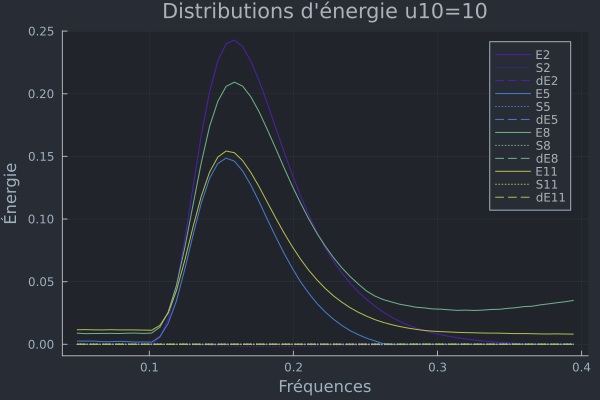
\includegraphics[width=0.8\linewidth]{Figures/figures/Spectral-tail.png}
\end{center}
\caption{\label{org580281b}Illustration du spectre d'énergie à divers points du domaine. Le spectre est à l'équilibre, mais on peut constater l'apparition de fortes trainées spectrales pour certains endroits.}
\end{wrapfigure}

Dans les observations sorties de mon modèle spectral en Julia, on note que la trainée spectrale (\emph{spectral tail}) prend de l'ampleur sur certains points de grille du domaines.
Par exemple, voir la figure \ref{org580281b} où le \(8^{\text{ème}}\) spectre d'énergie -- nommé « E8 » en vert -- augmente fortement autour de \(0.4\;\rad\cdot\mathrm{s}^{-1}\).
Dany, Eliot Bismuth et Sebastien Dugas ont eu le même problème, c'est pourquoi ils ont du rectifier le tir. Sebastien Dugas avait du coder un nouveau terme associé aux quadruplètes \autocite{Hasselmann_1962}, qui devrait se retrouver dans \href{https://semaphore.uqar.ca/id/eprint/1846/}{sa maîtrise}.\bigskip

En l'absence de glace, l'équation de balance d'énergie est donnée par

\begin{equation}
   \frac{1}{c_g} \dv{E}{t} = S_{in} + S_{ds} + S_{nl}.
\end{equation}
\subsubsection{Dissipation et \emph{whitecapping} (Retour rapide)}
\label{sec:orgce77660}
La dissipation d'énergie est généralement représentée de manière proportionelle à une puissance de l'énergie selon Dugas, soit
\begin{equation}
   S_{ds} \propto E^n.
\end{equation}
Selon Dugas, \(n=1\) dans la plupart des cas, mais certains modèles utilisent \(n =2,\pt 3,\pt\text{où même}\ 5\).
La représentation d'\Textcite{hasselmann1974spectral} est généralement la plus utilisée (Donc \(n=1\) avec un coefficient \(\gamma\) dépendant de plein de trucs (Voir le \href{Fichiers\_pdf/rapport-2024-07-26.pdf}{rapport du 26 juillet 2024}).
\subsubsection{Spectre de Pierson-Moskowitz (Retour rapide)}
\label{sec:orgb65fff7}
Dans le \href{rapport-2024-08-23.pdf}{rapport du 23 juillet}, nous ne savions pas d'où Bismuth tirait sa représentation du spectre JONSWAP, soit
\begin{equation}
\label{eq:org797fb6c}
   E_{JONSWAP}(\omega) = 0.2H_s^2 \qty(\frac{\omega_p^4}{\omega^5}) \exp{-\frac{5}{4}\qty(\frac{\omega_p}{\omega})^4} \times 3.3^{\exp{\frac{-(\omega-\omega_p)^2}{2\sigma^2 \omega_p^2}}},
\end{equation}
On ne savait pas vraiment d'où ça venait.
pourtant, Sebastien Dugas a réussi à trouver le lien entre le spectre de l'article de JONSWAP et l'utilisation de Bismuth (\ref{eq:org797fb6c}).
Normalement, nous devrions avoir le spectre de \Textcite{hasselmann1973measurements}, soit
\begin{align}
   && E_{JONSWAP}(f) = \alpha g^2 (2\pi)^4 f^{-5} \exp[- \frac{5}{4} \qty(\frac{f}{f_m})^{-4}]\times \gamma^{g(f,\sigma)}
   && \text{où}
   && g(f,\sigma) = \exp[ \frac{-(f-f_m)^2}{2\sigma^2f_m^2}]. &&
\end{align}
On sait maintenant que la version d'Eliot Bismuth (\ref{eq:org797fb6c}) est tirée de \Textcite[, à l'équation 11 de l'article]{goda1988variablity}.
Dans son article, ce dernier relie statistiquement la hauteur significative des vagues (ce qu'on appelle courament \(H_s\) ou \(H_{\sfrac{1}{3}}\)) avec le coefficient \(\alpha\), la fréquence du pique \(f_p\) et la valeur du champ gravitationnel \(g\) dans l'équation du spectre de JONSWAP.
\subsubsection{Désambiguation des quantités importantes}
\label{sec:org7579b80}

\begin{table}[htbp]
\caption{Quantités importantes dans le domaine d'étude des vagues et désambiguation des symboles utilisés.}
\centering
\begin{tabular}{lclc}
Description de la variable & Symbole & Description anglo & Source\\
\hline
\hline
\textbf{Hauteur significative des} & \(H_s\) & \emph{Significant wave height} & WMO (1998)\\
\textbf{vagues} & \(H_{\sfrac{1}{3}}\) &  & \Textcite{goda1988variablity}\\
\hline
\textbf{Période du maximum de} & \(T_p\) & \emph{Spectral peak period} & WMO (1998)\\
\textbf{fréquence} &  &  & \\
\hline
\textbf{Fréquence du maximum} & \(f_m\) & \emph{Peak frequency} & \Textcite{hasselmann1973measurements}\\
\textbf{(du pique)} & \(f_p\) & \emph{Wave frequency corresponding} & WMO (1998)\\
 &  & \emph{to the peak of the spectrum} & \\
\hline
 &  &  & \\
\end{tabular}
\end{table}
\subsubsection{Comment arriver aux quadruplettes}
\label{sec:orga04f757}

On peut utiliser les notes de \Textcite[Chap.4 \emph{Nonlinear wave–wave interactions and wave dissipation}]{Janssen2004chap4} pour simplifier la matière, mais mentionnons que tout a \emph{grosso modo} été fait par \Textcite{Hasselmann_1962}.
Je tiens à mentionner que les mathématiques sont extrpemement peu intuitives et que ça m'a pris quelques jours pour juste comprendre ce qu'on tente de dire. Je tiens donc à saluer le courage de Sebastien Dugas dans l'approche de ce problème. \bigskip

On peut diviser l'énergie du champ de vagues en deux quantités \autocite{Hasselmann_1962}
\begin{equation}
   E_\text{totale} = E_\text{kinétique} + E_\text{potentielle}.
\end{equation}
On peut dire que c'est le Hamiltonien de la surface de l'eau.
La partie potentielle sera décrite par l'élévation de la surface de l'eau, tandis que la partie kinétique sera représentée par une variable \(\phi\) qu'on appellera -- malheureusement -- le « potentiel » du champ de vitesse, décrit par \(\vb{u} = -\gradient{\phi}\).
Donc si l'on développe ça, on obtient le Hamiltonien \autocite{Janssen2004chap4},
\begin{equation}
\label{eq:org8b2bf8d}
   E = \frac{1}{2} \int\dd \xx \int_{-\infty}^\eta\dd z\, \qty( (\gradient{\phi})^2 + \qty(\pdv{\phi}{z})^2 ) + \frac{g}{2} \int \dd\xx\, \eta^2.
\end{equation}
Cette équation  (\ref{eq:org8b2bf8d}) décrit justement le transfert entre les deux composantes de l'énergie.
On veut donc connaître la forme de \(\phi\), c'est un peu ça le nerf de la guerre.
On sait que la solution pour \(\phi\) satisfait aussi l'équation de Laplace, soit
\begin{equation}
   \laplacian{\phi} + \pdv[2]{\phi}{z} = 0.
\end{equation}
Tandis que les conditions frontières satisfont 
\begin{equation}
    \phi(\xx, t, z = \eta) = \psi(\xx,t)  \qquad \text{et} \qquad \eval{\pdv{\phi}{z}}_{z\rightarrow-\infty} = 0.
\end{equation}
On peut aussi insérer la transformée de Fourier, définit comme
\begin{equation}
   \phi = \int\dd\vb{k}\, \hat{\phi}\, e^{i\vb{k}\cdot\xx}.
\end{equation}
Donc pour satisfaire la condition à l'infinit, il est évident que la solution dans le monde des « nombres d'onde »  est donnée par
\begin{equation}
\label{eq:org8e93cf6}
   \hat{\phi}(x, t, z) =  \hat{\phi}(t)\,e^{kz}.
\end{equation}
Là, comme le mentionne \Textcite{Janssen2004chap4}, il faut aussi satisfaire la condition à \(z=\zeta\), dans le monde de Fourier
\begin{equation}
   \phi(\xx,t,z = \eta) = \phi(\xx,t) = \int\dd\vb{k}\, \hat{\psi}\, e^{i\vb{k}\cdot\xx}
\end{equation}
et on peut faire du progrès en faisant une expansion en série de Taylor autour de \(z = 0\), soit
\begin{equation}
   \phi(\xx,z = \eta) = \phi(\xx,z=0) + \eta \pdv{}{z}\phi + \frac{\eta^2}{2}\pdv[2]{}{z}\phi + \cdots = \psi
\end{equation}
On fait la transformée de Fourier de tout ça et on réarrange, de sorte à obtenir
\begin{equation}
   \hat{\phi}(t,z=0) = \hat{\psi} - \fourier \qty[\eta \eval{\pdv{}{z}\phi}_{z=0} + \frac{\eta^2}{2}\eval{\pdv[2]{}{z}\phi}_{z=0} + \mathscr{O}(\geq3)].
\end{equation}
On substitue
\begin{align}
   \hat{\phi}(t,z=0) = \hat{\psi} - \fourier\bigg[&\qty(\int \dd\vb{k}\, \hat{\eta}\, e^{i\vb{k}\cdot\xx}) \cdot\eval{\qty(\pdv{}{z}\int\dd\vb{k}\,\hat{\phi}(z,t,k)\,e^{i\vb{k}\cdot\xx})}_ {z=0}\nonumber\\
   &+\frac{1}{2}\qty(\int \dd\vb{k}\, \hat{\eta}\, e^{i\vb{k}\cdot\xx})\cdot\qty(\int \dd\vb{k}\, \hat{\eta}\, e^{i\vb{k}\cdot\xx})\cdot \eval{\qty(\pdv[2]{}{z}\int\dd\vb{k}\,\hat{\phi}(z,t,k)\,e^{i\vb{k}\cdot\xx})}_{z=0}
   +\mathscr{O}(\geq3)\bigg].
\end{align}
Comme \(z\) et \(k\) sont des variables indépendantes et que les fonctions ne devraient pas avoir de discontinuités, on peut distribuer les dérivées.
Nous avons donc
\begin{align}
   \hat{\phi}(t,z=0) = \hat{\psi} - \fourier\bigg[&\qty(\int \dd\vb{k}\, \hat{\eta}\, e^{i\vb{k}\cdot\xx}) \cdot\qty(\int\dd\vb{k}\,\eval{\pdv{\hat{\phi}(z,t,k)}{z}}_{z=0}\,e^{i\vb{k}\cdot\xx})\nonumber\\
   &+\frac{1}{2}\qty(\int \dd\vb{k}\, \hat{\eta}\, e^{i\vb{k}\cdot\xx})\cdot\qty(\int \dd\vb{k}\, \hat{\eta}\, e^{i\vb{k}\cdot\xx})\cdot \qty(\int\dd\vb{k}\,\eval{\pdv[2]{\hat{\phi}(z,k,t)}{z}}_{z=0}\,e^{i\vb{k}\cdot\xx})
   +\mathscr{O}(\geq3)\bigg].
\end{align}
Puis on prend la solution \ref{eq:org8e93cf6} pour avoir
\begin{align}
   \hat{\phi}(t,z=0) = \hat{\psi}\, -& \fourier\bigg[\qty(\int \dd\vb{k}\, \hat{\eta}\, e^{i\vb{k}\cdot\xx}) \cdot\qty(\int\dd\vb{k}\eval{k\,\hat{\phi}(t)e^{kz}}_{z=0}\,e^{i\vb{k}\cdot\xx})\bigg]\nonumber\\
   -\frac{1}{2}&\fourier \bigg[\qty(\int \dd\vb{k}\, \hat{\eta}\, e^{i\vb{k}\cdot\xx})\cdot\qty(\int \dd\vb{k}\, \hat{\eta}\, e^{i\vb{k}\cdot\xx})\cdot \qty(\int\dd\vb{k}\eval{k^2 \hat{\phi}(t)e^{kz}}_{z=0}\,e^{i\vb{k}\cdot\xx})
   +\mathscr{O}(\geq3)\bigg].
\end{align}
Puis finalement, on applique les transformée de Fourier, soit
\begin{align}
   \hat{\phi}(t,z=0) = \hat{\psi}\, -& \int\dd\xx\bigg[\qty(\int \dd\vb{k}\, \hat{\eta}\, e^{i\vb{k}\cdot\xx}) \cdot\qty(\int\dd\vb{k}\, k\,\hat{\phi}(t)\,e^{i\vb{k}\cdot\xx})\,e^{-i\vb{k}\cdot\xx}\bigg]\nonumber\\
   -\frac{1}{2}&\int\dd\xx \bigg[\qty(\int \dd\vb{k}\, \hat{\eta}\, e^{i\vb{k}\cdot\xx})\cdot\qty(\int \dd\vb{k}\, \hat{\eta}\, e^{i\vb{k}\cdot\xx})\cdot \qty(\int\dd\vb{k}\,k^2 \hat{\phi}(t,k)\,e^{i\vb{k}\cdot\xx})e^{-i\vb{k}\cdot\xx}
   +\cdots\bigg].
\end{align}
Puis, c'est là qu'on redistribue tout
\begin{align}
   \hat{\phi}(t,z=0,\vb{k}) = \hat{\psi}(k,t)\, -& \int\dd\xx\qty[\iint\dd\vb{k}_{1,2}\qty( \hat{\eta_1}\, \,k_2\,\hat{\phi}_2\,e^{i(-\vb{k} + \vb{k_1}+\vb{k}_2)\cdot\xx})]\nonumber\\
   +\frac{1}{2}&\int\dd\xx \qty[\iiint \dd\vb{k}_{1,2,3}\qty( \hat{\eta}_1\hat{\eta}_2  k_3^2 \hat{\phi}_3\,e^{i(-\vb{k} + \vb{k}_1+\vb{k}_2+\vb{k}_3)\cdot\xx}) ]    + \cdots
\end{align}
Là, la définition du delta de Dirac (voir ce \href{https://math.stackexchange.com/questions/1343859/why-does-integrating-a-complex-exponential-give-the-delta-function}{Stack Exchange}), c'est
\begin{equation}
   \var(x) = \frac{1}{2\pi} \int_{-\infty}^\infty e^{ikx} \dd k,
\end{equation}
et l'analogue en 2d existe aussi et c'est comme ça qu'on réussit à se débarrasser de la composante en \(x\).
Mentionnons que une des propriétés importante de la fonction delta de Dirac, soit
\begin{equation}
   \iint \dd\xx f(\xx) \delta(\xx - \xx_0) = f(\xx_0),
\end{equation}
donc on obtient
\begin{align}
   \hat{\phi}(t,z=0,\vb{k}) = \hat{\psi}(k,t)\, -& \iint\dd\vb{k}_{1,2}\qty( \hat{\eta_1}\, \,k_2\,\hat{\phi}_2\cdot \var(\vb{k}-\vb{k}_1-\vb{k}_2))\nonumber\\
   +\frac{1}{2}&\iiint \dd\vb{k}_{1,2,3}\qty( \hat{\eta}_1\hat{\eta}_2  k_3^2 \hat{\phi}_3 \cdot\var(\vb{k} - \vb{k}_1 - \vb{k}_2 - \vb{k}_3))    + \cdots
\end{align}
étant donné que \(\var(x) = \var(-x) = -\var(x)\).\bigskip

On y est presque, mais je n'y arrive pas et ça fait trois jours que je travaille là-dessus.
Il faudra donc mettre mon énergie ailleurs\ldots{}

\printbibliography
\end{document}
